\documentclass[a4paper]{article}

\usepackage[T2A]{fontenc}
\usepackage[russian]{babel}
\usepackage{graphicx}
\usepackage{float}
\usepackage{hyperref}
\usepackage{amsmath, amssymb}
\usepackage{caption}
\usepackage{geometry}
\usepackage{pdfpages}
\usepackage[normalem]{ulem}
\usepackage{mathtools}
\usepackage{diffcoeff}

\geometry{top=2cm,bottom=2cm,left=2cm,right=2cm}

\newcommand{\minus}{\scalebox{0.75}[1.0]{$-$}}


\date{}

\begin{document}

\begin{center}
\textsc{Санкт-Петербургский национальный исследовательский институт информационных технологий, механики и оптики\\[3mm]
Физический факультет} \\[3mm]

\end{center}
\vspace{5mm}
\line(1,0){\textwidth}
\begin{center}
\textbf{ЛАБОРАТОРНАЯ РАБОТА №1.10\\}
\textbf{"Исследование вынужденных
крутильных колебаний с регулируемым
затуханием с помощью маятника Поля"}
\end{center}
\vspace{2mm}
\line(1,0){\textwidth}
\vspace{5mm}
\begin{minipage}{0.4\textwidth}
    Группа: Z3144 \\
    Студент: Евгений Турчанин\\
    \vspace{1mm}
\end{minipage}
\hfill
\vspace{1mm}
\line(1,0){\textwidth}



\section{\textbf{Цель}}

Изучение характеристик свободных и вынужденных колебаний на примере маятника Поля.

\section{\textbf{Задачи}}

\begin{enumerate}
	\item Опредление периода колебаний маятника.
	\item Исследование свободных затухающих колебаний.
	\item Исследование вынужденных колебаний.
\end{enumerate}

\section{\textbf{Теоретическое введение}}
Свободные колебания
Рассмотрим физическую систему, находящуюся в состоянии
устойчивого равновесия. Если ее вывести из этого состояния
каким-либо внешним воздействием и затем предоставить самой
себе, при определенных условиях в системе будут происходить
колебания около положения равновесия. Такие колебания называются собственными или свободными. Любая система, способная совершать свободные колебания, называется осциллятором.
Физически осциллятор может быть реализован самыми разными
способами. Это может быть маятник, груз, подвешенный на пружине, электромагнитный LCR-контур и т. д. Для механического
осциллятора наличие трения, неизбежного в любой реальной механической системе, приводит к тому, что собственные колебания
постепенно затухают из-за диссипации (рассеяния) механической
энергии, и, в конце концов, система приходит в состояние покоя
в положении равновесия.\\
В данной работе в качестве осциллятора используется торсионный пружинный осциллятор (маятник Поля), представляющий собой уравновешенный маховик со спиральной пружиной
(рис. 1). Один конец пружины прикреплен к маховику, другой
– закреплен неподвижно. При повороте маховика из положения
равновесия пружина закручивается или раскручивается и создает
момент силы, заставляющий маховик возвращаться к положению
равновесия. Подобное устройство используется в механических
карманных или наручных часах.
\begin{figure}[H]
	\begin{center}
		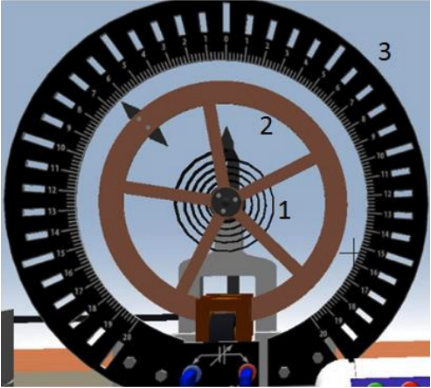
\includegraphics[scale=0.3]{pick_1.png}
		\caption{Маятник Поля. 1 - пружина, 2 - ротор, 3 - угловая шкала}
	\end{center}
\end{figure}

При повороте маховика из положения равновесия на угол $\varphi$
прикрепленная к нему спиральная пружина создает возвращающий момент $M$ , пропорциональный углу отклонения:
\begin{equation}
	M=-D\varphi
\end{equation}

Коэффициент пропорциональности $D$ в этой формуле называется угловой жесткостью пружины.\\
Второй закон Ньютона для вращательного движения маховика
в отсутствие сил трения с учетом выражения (1) принимает вид:
\begin{equation}
	I\ddot{\varphi}=-D\varphi
\end{equation}
где $I$ – момент инерции маховика. Здесь, как это принято в
механике, производная по времени обозначена точкой, т. е. $\ddot{\varphi}=\diff[2]\varphi t$
Введем обозначение $\omega_0^2=\dfrac{D}{T}$
 и преобразуем дифференциальное
уравнение (2) к стандартному виду
\begin{equation}
	\ddot{\varphi}+\omega_0^2\varphi=0
\end{equation}
Решение уравнения (3) представляет собой гармоническое колебание:
\begin{equation}
\varphi=C_1\cos{\omega_0 t}+C_2\sin{\omega_0 t}=A_0\cos{(\omega_0 t+\varphi_0)}
\end{equation}
Здесь величина $A_0$ называется начальной амплитудой , $\omega_0$ –
собственной циклической (угловой) частотой, $\varphi_0$ – начальной фазой колебаний.\\
Произвольные постоянные $C_1$ и $C_2$ либо выражающиеся через
них амплитуда $A_0$ и начальная фаза $\varphi_0$ в решении (4) зависят
от начальных условий, т. е. от угла отклонения $\varphi_0$ и угловой
скорости $\dot{\varphi}(0)$ при $t$ = 0. Другими словами, эти характеристики
колебательного движения зависят от способа возбуждения колебаний.\\
Колебания происходят с угловой частотой $\omega_0$, квадрат которой
пропорционален жесткости пружины $D$ и обратно пропорционален моменту инерции $I$ маховика. Частота $\omega_0$ и соответствующий
ей период $T_0=\dfrac{2\pi}{\omega_0}$
$\omega_0$ , в отличие от амплитуды и начальной фазы,
не зависят от начальных условий – они целиком определяются свойствами самого осциллятора, т. е. значениями параметров
осциллятора $D$ и $I$.\\

Осциллятор, поведение которого описывается дифференциальным уравнением вида (3), называется линейным (поскольку возвращающая сила пропорциональна величине отклонения от равновесия). Собственные колебания линейного осциллятора всегда
происходят с одной и той же собственной частотой $\omega_0$ независимо от способа возбуждения. Независимость частоты собственных
колебаний от начальных условий, а, следовательно, от амплитуды (и энергии) колебаний называют изохронностью линейного
осциллятора.
При наличии силы вязкого трения во втором законе Ньютона
для вращательного движения маховика необходимо учесть тормозящий момент этой силы, пропорциональный угловой скорости
ротора $\dot{\varphi}$. В этом случае дифференциальное уравнение, описывающее движение маховика имеет вид
\begin{equation}
	\ddot{\varphi}+2\beta\dot{\varphi}+\omega_0^2\varphi=0
\end{equation}

где коэффициент затухания характеризует интенсивность вязкого трения в системе. Коэффициент затухания $\beta$ имеет размерность частоты.\\
Если трение невелико и $\beta<\omega_0$, общее решение дифференциального уравнения (5) имеет колебательный характер и может
быть представлено в следующем виде:
\begin{equation}
	\varphi(t)=A_0\exp{[-\beta t]}\cos\left(\omega_1 t+\varphi_0\right)
\end{equation}

Это решение описывает затухающие колебания, амплитуда которых $A(t)=A_0\exp{[-\beta t]}$ экспоненциально убывает со временем. Начальные значения амплитуды $A_0$ и фазы $\varphi_0$ определяются из начальных условий. Циклическая (угловая) частота $\omega_1$ затухающих
колебаний дается следующим выражением:
\begin{equation}
	\omega_1=\sqrt{\omega_0^2-\beta^2}=\omega_0\sqrt{1-(\beta/\omega_0)^2}
\end{equation}
График затухающих колебаний (6) показан на рис. 2.
\begin{figure}[H]
	\begin{center}
		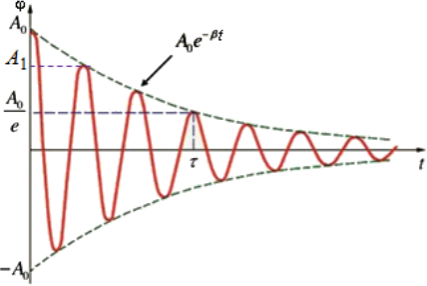
\includegraphics[scale=0.3]{pick_2.png}
	\end{center}
	\caption{Затухающие колебания}
\end{figure}

За время $\tau=1/\beta$ амплитуда колебаний уменьшается в $e$ =
2.72 раз. Это время $\tau$ называется временем затухания колебания. Для характеристики быстроты затухания колебаний используют, наряду с размерным коэффициентом $\beta$ (или временем
затухания $\tau$ ), также безразмерные параметры.
Логарифмический декремент затухания $\lambda$: логарифм отношения последовательных максимальных отклонений в одну сторону:
\begin{equation}
	\lambda=\ln{(A_n/A_{n+1})}=\beta T=T/\tau
\end{equation}
где $A_n$ – амплитуда затухающего колебания через n периодов
после старта.\\
График функции
\begin{equation}
	f(t)=\ln{A_0/A(t)}
\end{equation}
имеет вид прямой с коэффициентом наклона $\beta$. Если же время
измерять не в секундах, а в периодах, то коэффициент наклона
будет равен $\lambda$. График функции $f(t)$, соответствующий колебанию, показанному на рис. 2 с периодом $T$ = 1.5 с, показан на рис. 3
\begin{figure}[H]
\begin{center}
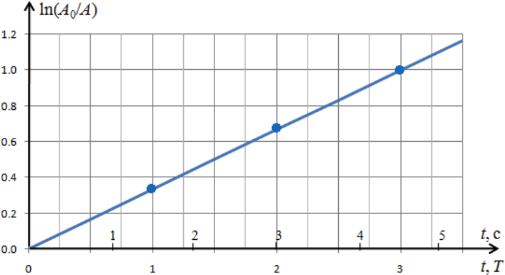
\includegraphics[scale=0.4]{pick_3.png}
\caption{График для нахождения $\beta$ и $\lambda$}
\end{center}
\end{figure}
Обратная логарифмическому декременту величина – это число колебаний, совершаемых осциллятором за время затухания $\tau$ .
Другой важной характеристикой колебательной системы является добротность $Q$:
\begin{equation}
	Q=\dfrac{\omega_0}{2\beta}
\end{equation}

При малом затухании ($\beta<\omega_0, T\approx T_0$) добротность связана с
логарифмическим декрементом как
\begin{equation}
	Q=\dfrac{\pi}{\lambda}
\end{equation}
и может быть интерпретирована как отношение запаса энергии в
системе к потерям энергии за период.\\
При сильном затухании ($\beta \leq \omega_0$) система после начального
возбуждения возвращается в положение равновесия, не совершая колебаний. При этом маховик либо асимптотически приближается к положению равновесия с одной стороны (рис. 4, а,
б), либо только один раз пересекает среднее положение и затем
приближается к нему с другой стороны (рис. 4, в). Последний
случай возможен, если при возбуждении отклоненный из положения равновесия ротор получает достаточно большую начальную
скорость в направлении положения равновесия.\\
Если $\beta=\omega_0$, затухание называют критическим. В критическом режиме добротность осциллятора $Q=0.5$, а величины $\tau$
и $\lambda$ теряют физический смысл. В этом случае общее решение
дифференциального уравнения (5) принимает следующий вид:
\begin{equation}
	\varphi=(C_1t+C_2)\exp{[-\beta t]}
\end{equation}
где константы $C_1$ и $C_2$ определяются из начальных условий.
\begin{figure}[H]
	\begin{center}
	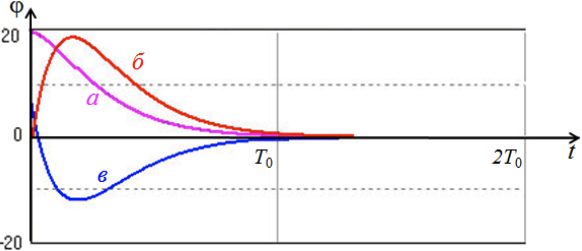
\includegraphics[scale=0.4]{pick_4.png}
	\caption{Поведение системы с критическим затуханием в зависимости
	от начальных условий:\\
$\text{} \hspace{95pt} a-\varphi_0=20, \; \dot{\varphi}=0, \; \varphi_0=0, \; \dot{\varphi}=0.9\omega_0; \: -\varphi_0=10, \; \dot{\varphi}=-0.9\omega_0$}
	\end{center}
\end{figure}
Система с критическим затуханием после начального возбуждения возвращается в состояние покоя быстрее, чем при любом другом значении коэффициента затухания $\beta$. Это свойство
используется, например, в стрелочных измерительных приборах
для того, чтобы при изменении измеряемого параметра стрелка
быстрее переходила в новое положение, не совершая колебаний.
Затухание, близкое к критическому, преднамеренно вводится также в амортизационную систему автомобиля для предупреждения
раскачки кузова на неровностях дороги.

\textbf{Вынужденные колебания}\\
Рассмотрим теперь движение осциллятора под действием синусоидальной вынуждающей силы. Для маятника Поля такая ситуация реализуется через присоединение ранее неподвижного конца пружины к шатуну, совершающему колебательное движение.\\
Пусть точка соединения шатуна с пружиной принудительно совершает гармонические колебания с некоторой амплитудой $\theta_0$ и угловой частотой $\omega$, так что угол отклонения точки соединения
от среднего положения $\theta(t)$ зависит от времени по закону:
\begin{equation}
\theta(t)=\theta_0\sin{\omega t}
\end{equation}
Если в некоторый момент времени $t$ маховики конец пружины, соединенный с ним, отклонен от среднего положения на угол $\varphi$, а второй конец пружины, соединенный с шатуном, в
этот момент смещен от среднего положения на угол $\theta$, то со
стороны пружины на маховик действует момент сил $M=D(\varphi-\theta)=D\varphi-D\theta_0\sin{(\omega t)}$. Этот момент силы отличается от момента (1) дополнительным слагаемым $D\theta_0\sin{(\omega t)}$, т. е. на маховик
действует дополнительный периодический момент вынуждающей
силы $D\theta_0\sin{(\omega t)}$. Соответственно дифференциальное уравнение
движения осциллятора вместо (5) запишется как
\begin{equation}
	\ddot{\varphi}+2\beta\dot{\varphi}+\omega_0^2=\omega_0^2\theta_0\sin{(\omega t)}
\end{equation}
В течение некоторого времени после включения внешней силы
(на протяжении переходного процесса) осциллятор успевает «забыть» свое начальное состояние: колебания осциллятора приобретают стационарный характер, и осциллятор совершает незатухающие синусоидальные колебания на частоте внешнего воздействия – так называемые установившиеся вынужденные колебания. Эти установившиеся колебания описываются периодическим
частным решением уравнения (14):
\begin{equation}
	\varphi(t)=a\sin{(\omega t+\delta)}
\end{equation}
Установившиеся колебания характеризуются определенными постоянными значениями амплитуды $a$ и сдвига фаз $\delta$ между колебаниями угла отклонения маховика и момента вынуждающей
силы. Величины $a$ и $\delta$ зависят от близости частоты внешнего
воздействия $\omega$ к собственной частоте осциллятора $\omega_0$. Зависимости $a(\omega)$ и $\delta(\omega)$ от частоты внешнего воздействия называют соответственно амплитудно-частотной и фазово-частотной характеристиками осциллятора (АЧХ и ФЧХ)
\begin{equation}
	a(\omega)=\dfrac{\omega_0^2\theta_0}{\sqrt{\omega_0^2-\omega^2}}\\
\end{equation}
\begin{equation}
	\tg \delta(\omega)=-\dfrac{2\beta\omega}{\omega_0^2-\omega^2}
\end{equation}
Для вынужденных колебаний при слабом затухании ($\beta\ll\omega_0$)
характерно явление резонанса – резкого возрастания амплитуды
установившихся колебаний при приближении частоты вынуждающей силы к собственной частоте осциллятора. При слабом затухании из (16) следует, что резонансная частота $\omega_{\text{рез}}\approx\omega_0$, а резонансная амплитуда
\begin{equation}
	a_{max}\approx Q\cdot\theta_0
\end{equation}
Поскольку из (16) следует, что при $\omega\to0$, добротность можно найти по отношению амплитуды колебаний при резонансе к амплитуде колебаний при очень низкой частоте вынуждающего воздействия:
\begin{equation}
	Q=\dfrac{a(\omega_0)}{a(\omega\to0)}
\end{equation}
С другой стороны из той же формулы (16) легко получить, что амплитуда вынужденных колебаний уменьшается в $\sqrt 2$ раз
по сравнению с резонансной при частотах возбуждения $\omega_{1, 2}=\omega_0 \pm \beta$
. Отсюда следует, что добротность можно также найти из
ширины резонансной кривой $\Delta\omega$ на уровне $1/\sqrt 2$ от максимума (см. формулу (10))

\begin{equation}
	Q=\dfrac{\omega_0}{\Delta \omega}
\end{equation}

Графики АЧХ и ФЧХ для разных значений добротности представлены на рис. 5

\begin{figure}[H]
\begin{center}
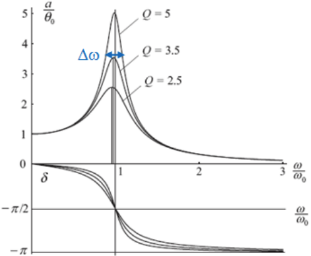
\includegraphics[scale=0.3]{pick_5.png}
\caption{AЧХ и ФЧХ осцилляторов с малым затуханием}
\end{center}
\end{figure}
При малом трении амплитуда $a(\omega)$ установившихся вынужденных колебаний осциллятора превышает угловую амплитуду $\theta_0$
конца шатуна при всех частотах в интервале между $\omega=0$ и
$\omega=\sqrt{2}\omega_0$. При больших частотах амплитуда осциллятора становится меньше амплитуды $\theta_0$ и стремится к нулю при дальнейшем
увеличении частоты – инертный маховик не успевает следовать
за быстрыми колебаниями момента вынуждающей силы.\\
Из графиков ФЧХ в нижней части рис. 5 видно, что установившиеся колебания всегда отстают по фазе от момента вынуждающей силы, поскольку сдвиг фаз $\delta(\omega)$ отрицателен при всех частотах.\\
Вдали от резонанса при низкой частоте $\omega \ll \omega_0$ запаздывание почти исчезает, т. е. маховик совершает колебания в фазе с
концом шатуна. В случае $\omega = \omega_0$ при любом трении колебания
маховика отстают от колебаний точки соединения шатуна и пружины на четверть периода ($\delta = -\pi/2$): когда маховик достигает
крайних отклонений, шатун проходит через среднее положение, и
наоборот. Когда $\omega$ значительно превосходит $\omega_0$, сдвиг фаз $\delta$ приближается к $-\pi$: запаздывание маховика по фазе составляет почти $2\pi$. В этом случае маховик и конец шатуна в любой момент
движутся в противоположных направлениях. Они почти одновременно проходят свои средние положения, и почти одновременно достигают своих противоположных крайних положений.





\section{\textbf{Экспериментальная установка}}
Схема установки показана на рис. 6, а ее внешний вид – на
рис. 7.
\begin{figure}[H]
\begin{center}
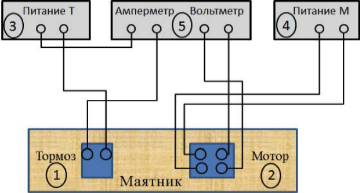
\includegraphics[scale=0.5]{pick_6.png}
\caption{Схема установки. 1 – электромагнитный тормоз, 2 - мотор, 3
– блок питания тормоза, 4 – блок питания мотора; 5 –
измерительный блок.}
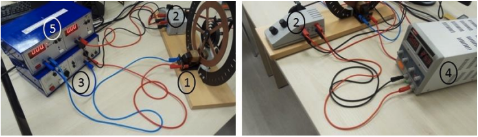
\includegraphics[scale=0.5]{pick_7.png}
\caption{Внешний вид установки. Обозначения как на рис. 6.}
\end{center}
\end{figure}
Для создания регулируемой силы вязкого трения используется
электромагнитный тормоз 1. Сила трения в таком тормозе пропорциональна скорости движения ротора маятника. Коэффициент
трения регулируется путем изменения тока $I_T$ через тормоз. Ток измеряется амперметром, расположенным в измерительном блоке 5.\\
Мотор 2, соединенный через кривошипно-шатунный механизм
с маятником, служит для возбуждения вынужденных колебаний.
Частота вращения мотора зависит от величины подаваемого напряжения. Это напряжение регулируется двумя ручками на корпусе мотора (рис. 8): верхняя ручка – грубая регулировка, нижняя ручка – точная. Напряжение на моторе измеряется вольтметром, расположенным в измерительном блоке 5.
\begin{figure}[H]
\begin{center}
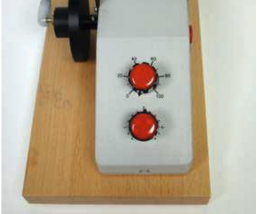
\includegraphics[scale=0.5]{pick_8.png}
\caption{Регулировка частоты вращения мотора}
\end{center}
\end{figure}


\section{\textbf{Данные}}


\begin{figure}[H]
\begin{center}
	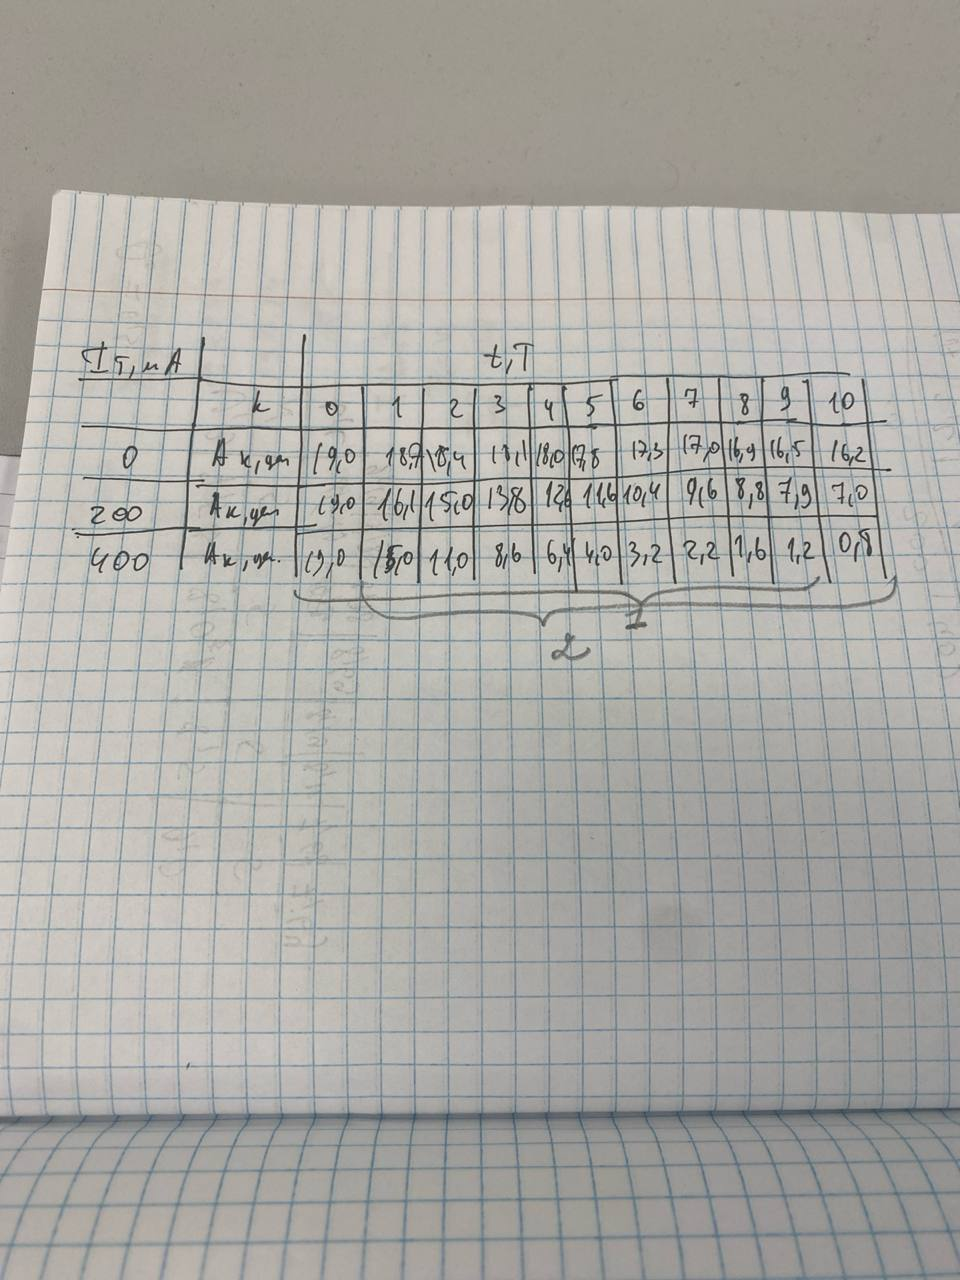
\includegraphics[scale=0.15]{data_1.png}
	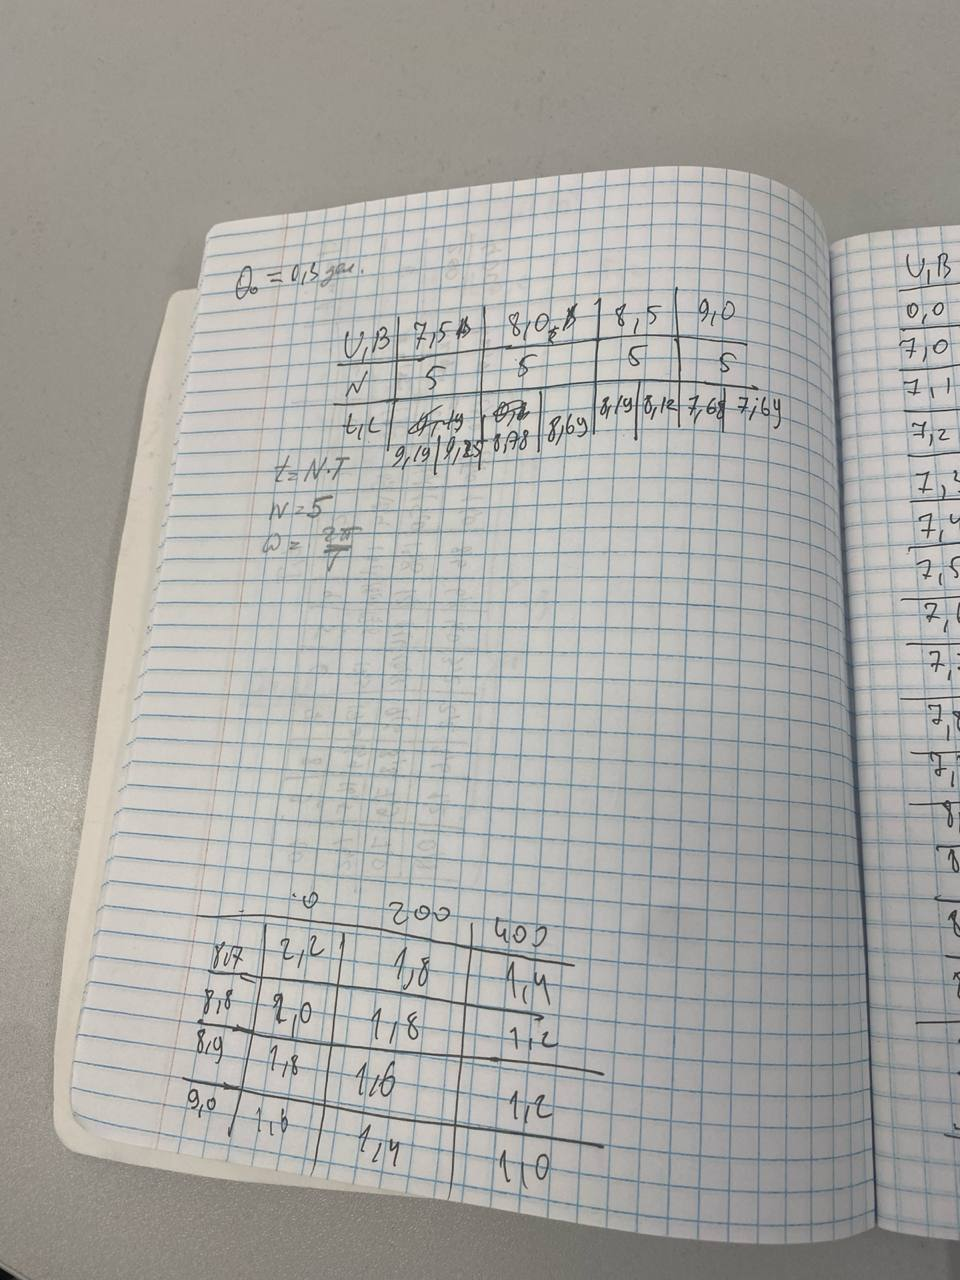
\includegraphics[scale=0.15]{data_2.png}
	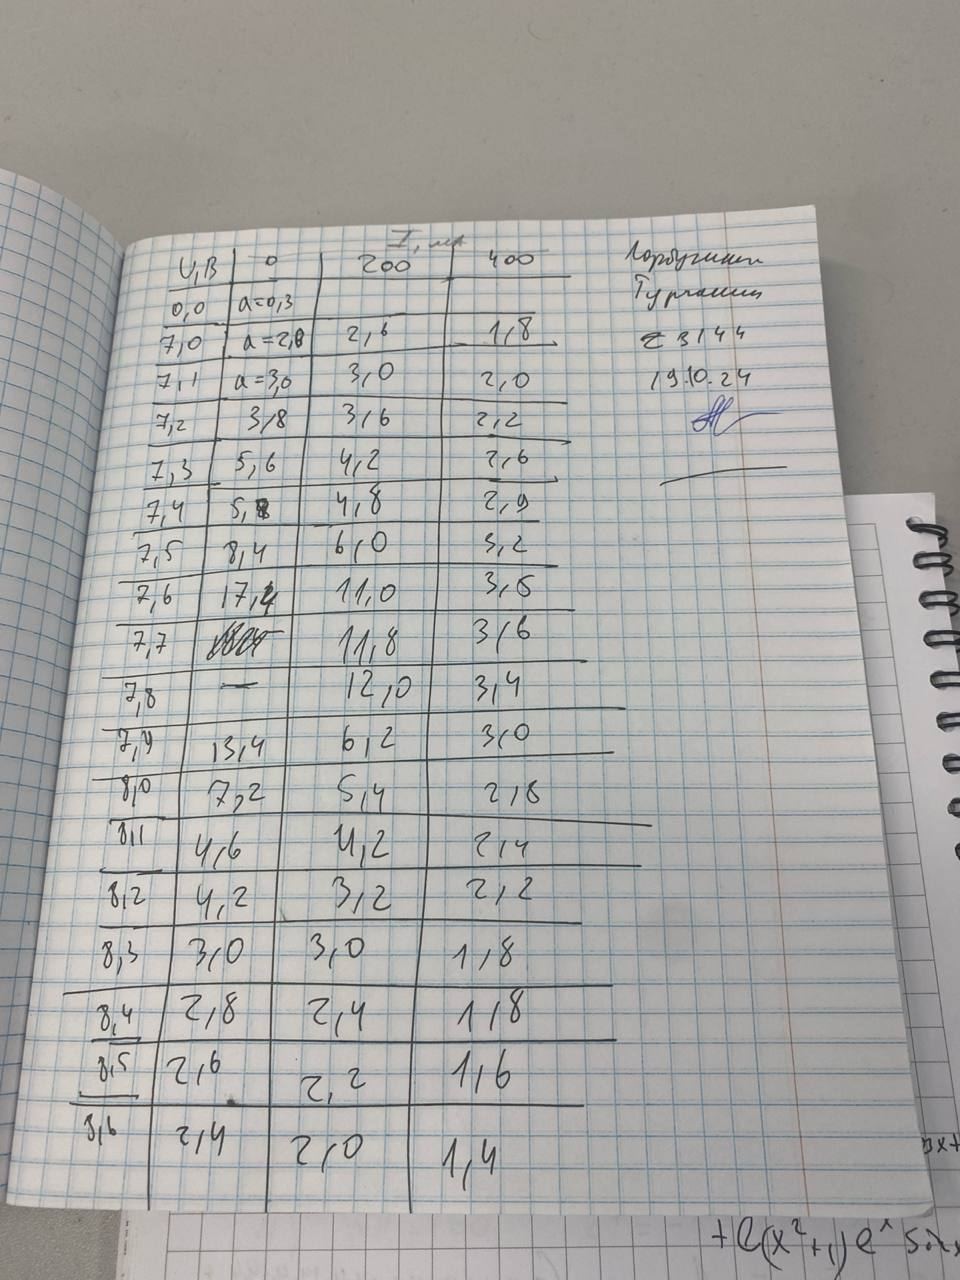
\includegraphics[scale=0.15]{data_3.png}
\end{center}
\end{figure}





\section{Результаты}


Средний период: $T_{mean}=17.6 \pm 0.51$c, циклическая частота: $\omega_{mean}=3.56 \pm 0.10$
\begin{figure}[H]
\begin{center}
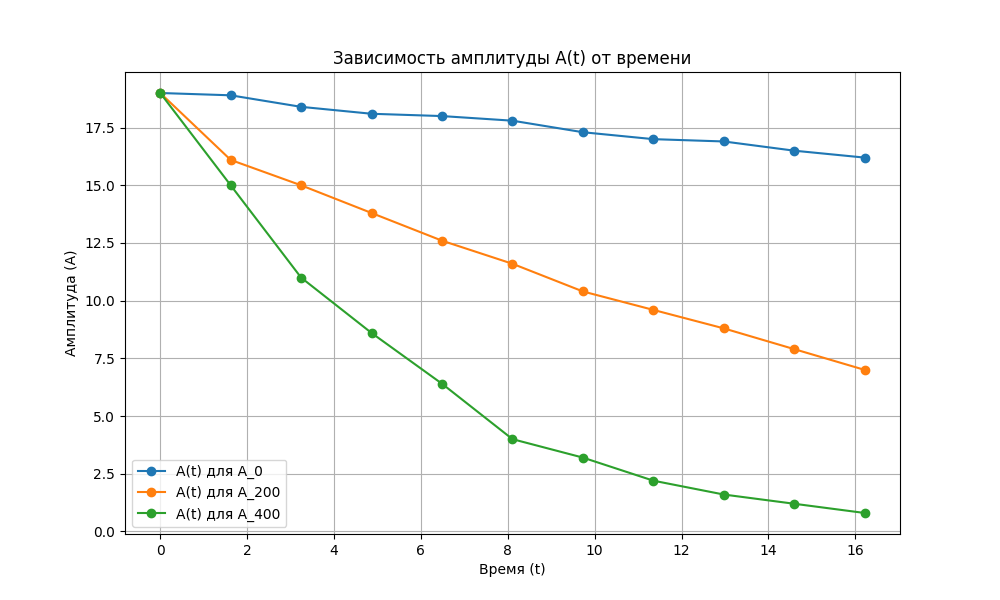
\includegraphics[scale=0.5]{gra_2.png}
\end{center}
\end{figure}
\centering
Среднее значение $\lambda$ для $A_0$: 0.01594\\
Среднее значение $\lambda$ для $A_{200}$: 0.099\\
Среднее значение $\lambda$ для $A_{400}$: 0.316\\
Среднее значение $Q$ для $A_0$: 197.054\\
Среднее значение $Q$ для $A_{200}$: 31.462\\
Среднее значение $Q$ для $A_{400}$: 9.918\\
Коэффициент затухания $\beta$ для $f(t)$ для $A_0$: 0.0099\\
Коэффициент затухания $\beta$ для $f(t)$ для $A_{200}$: 0.058\\
Коэффициент затухания $\beta$ для $f(t)$ для $A_{400}$: 0.197\\
\begin{figure}[H]
\begin{center}
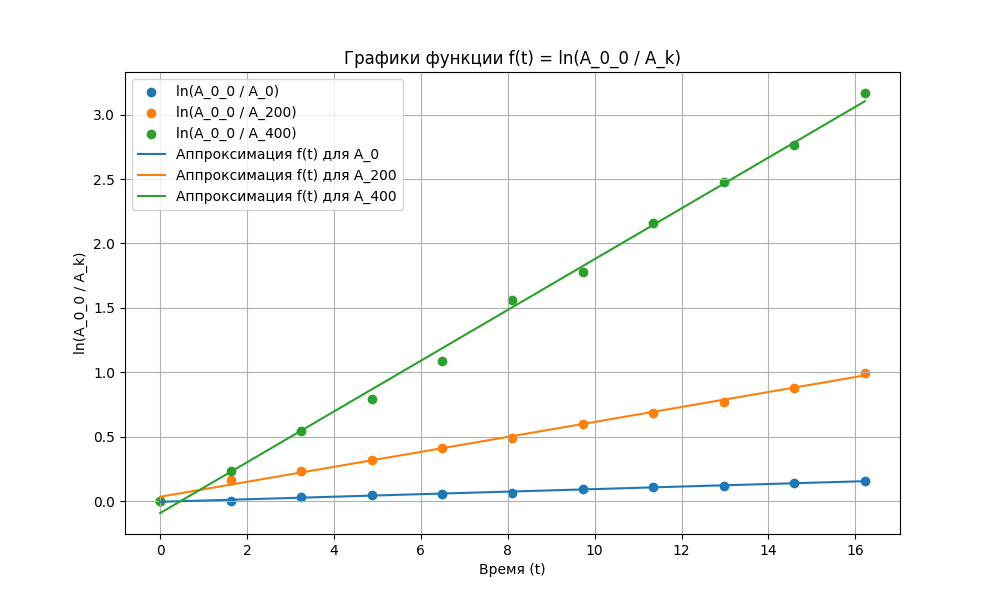
\includegraphics[scale=0.5]{gra_1.png}
\end{center}
\end{figure}
\begin{figure}[H]
\begin{center}
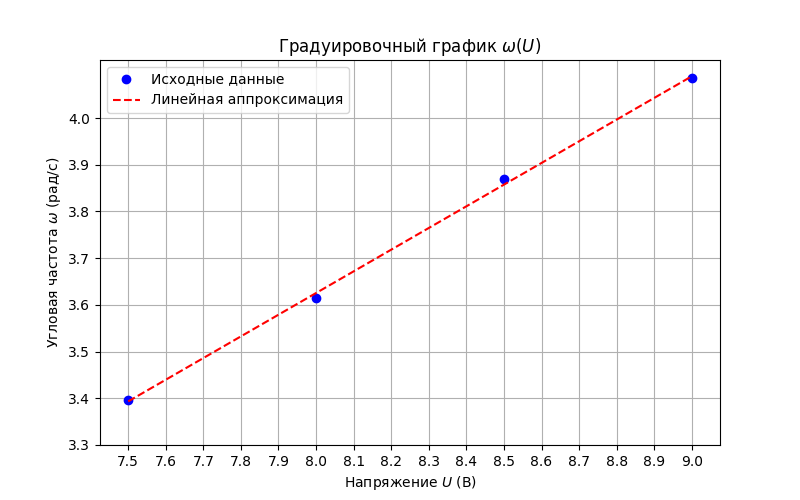
\includegraphics[scale=0.5]{gra_3.png}
\end{center}
\end{figure}



\begin{figure}[H]
\begin{center}
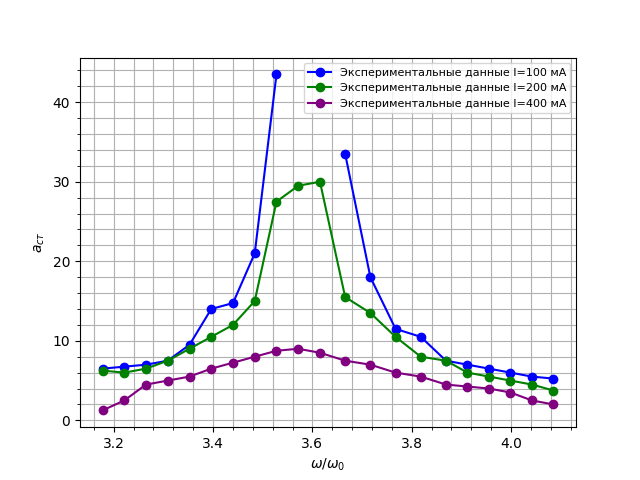
\includegraphics[scale=0.5]{gra_4.png}
\end{center}
\end{figure}


\begin{figure}[H]
\begin{center}
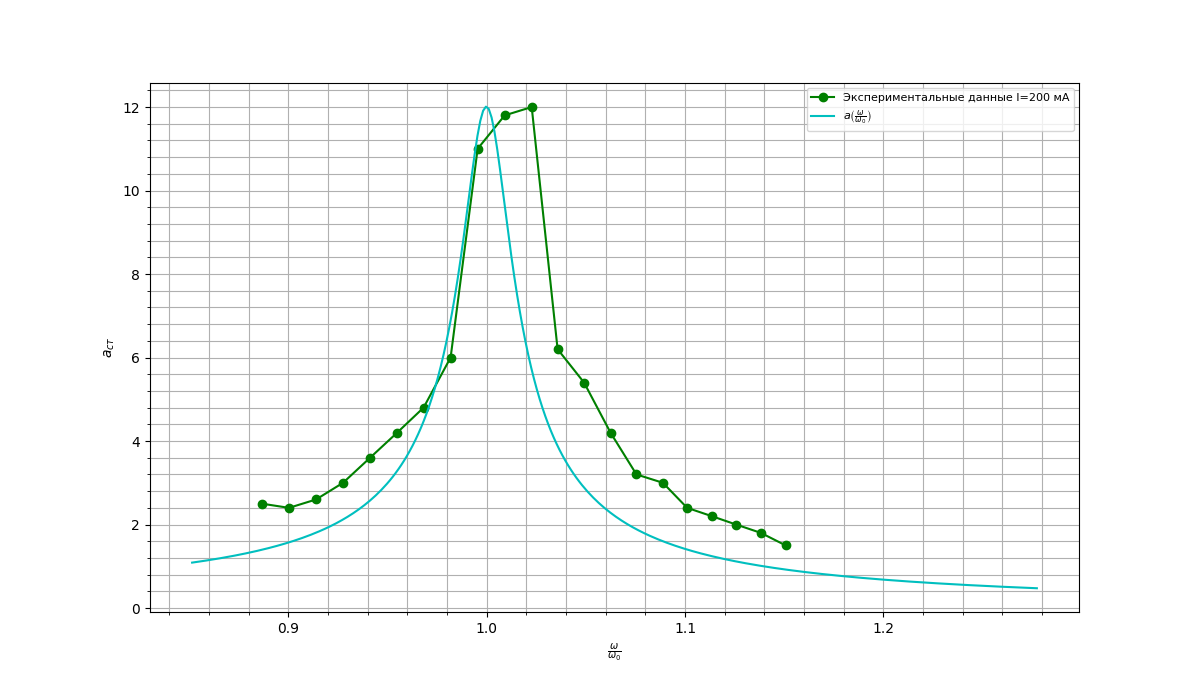
\includegraphics[scale=0.5]{gra_6.png}
\end{center}
\end{figure}

По АЧХ $Q \approx 30$, выше $Q=31.462$
\section{\textbf{Вывод}}



Из результатов можно сделать вывод, что теория совпадает с экспериментальными данными. Малые отклонения могут быть вызваны несколькими причинами:
\begin{enumerate}
	\item Неточность при измерении амплитуды
	\item При малых сопротивлениях тормоза, в моменты резонанса стрелка маятника выходила за шкалу для измерения амплитуды
	\item Человеческая реакция, тк для измерения периода использовался ручной таймер
\end{enumerate}




\end{document}



